
\subsection{Zyklische Belastung}

\begin{frame}
\frametitle{Szenarien}

\begin{tabular}{ll} 
%\toprule
\textbf{Erdbeben} & \textbf{Technische Vorgänge (Maschinen, Verkehr)} \\[2mm] 
%\midrule 
breites Frequenzspektrum  & diskretes Frequenzspektrum  \\[1mm] 
niedrige Frequenzen& hohe Frequenzen\\
($0.5 \dots 10$\,Hz)  & (bis kHz-Bereich) \\[1mm] 
wenige Sekunden  & langanhaltend \\[1mm] 
wenige Zyklen & viele Zyklen \\[1mm] 
verschiebungsgesteuert & kraftgesteuert \\[1mm] 
große Verformungen& kleine Verformungen\\
(starke Erdbeben) & (Normalbetrieb) 
%\bottomrule
\end{tabular}

\end{frame}

\begin{frame}
\frametitle{Begriffe}
Als \textsl{zyklisch} werden diejenigen wiederholten Belastungen definiert, 
bei denen Trägheitseffekte vernachlässigt werden können, andernfalls werden sie als
\textsl{transient} oder \textsl{dynamisch} bezeichnet.

\bigskip

\textsl{Nichtlineares} Verhalten tritt in den meisten Böden auf, 
sobald die Dehnungen größer als ca. $\varepsilon=10^{-5}$ werden. 

\bigskip

Das nichtlineare Verhalten von Böden unter zyklischer Belastung ist kompliziert 
und soll zunächst nur phänomenologisch beschrieben werden.
\end{frame}

\begin{frame}
\frametitle{Dehnungsgesteuerte Belastung}
\begin{figure}
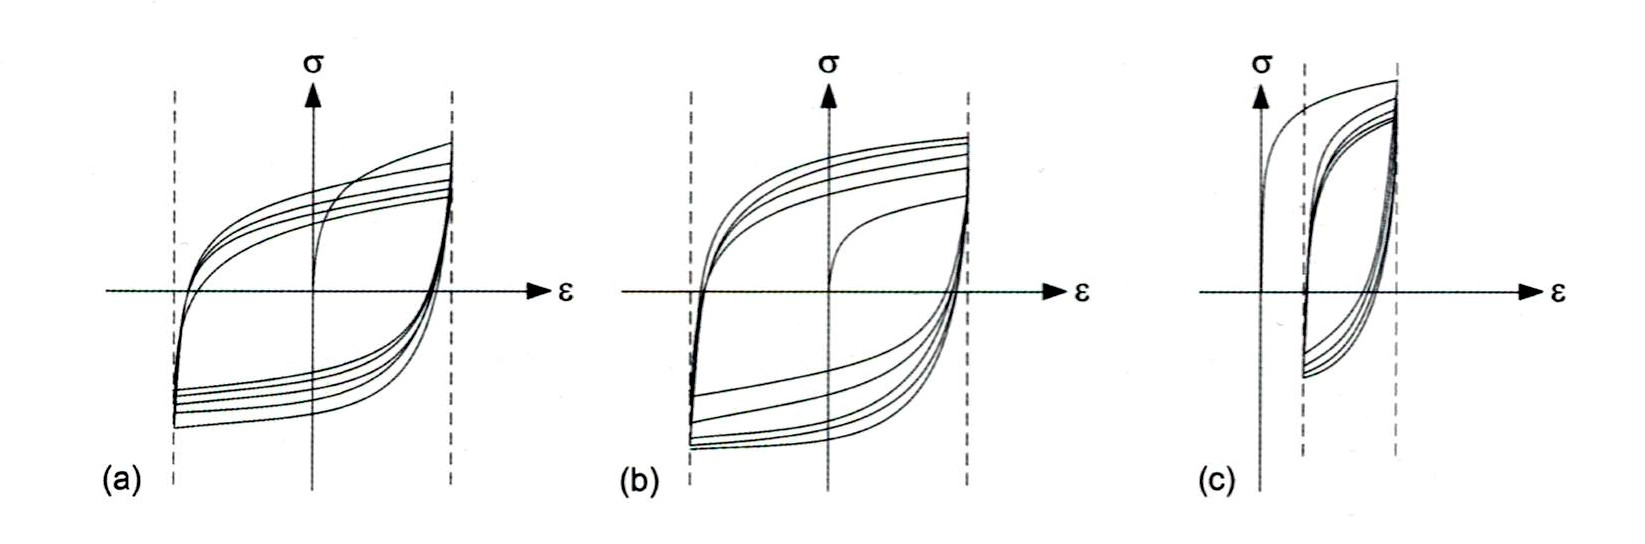
\includegraphics[width=\linewidth]{fig_img/bild14abc.jpg}
\caption*{(a) Entfestigung, (b) Verfestigung, (c) Relaxation der Mittelspannung \cite{Vrettos2017}} 
\end{figure}
Das Verhalten ist vorwiegend durch die Vorgeschichte bestimmt.
\end{frame}

\begin{frame}
\frametitle{Spannungsgesteuerte Belastung}
\begin{figure}
\centering
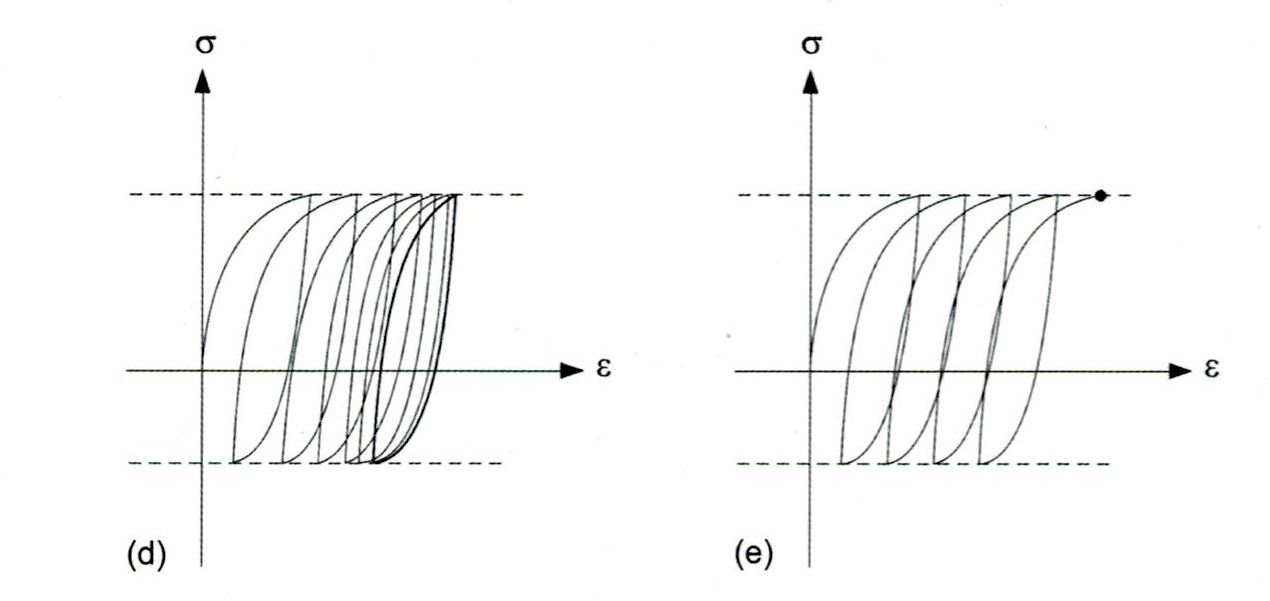
\includegraphics[width=0.75\linewidth]{fig_img/bild14de.jpg}
\caption*{(d) Einspielen (Shakedown), (e) unbegrenztes Anwachsen plastischer Dehnungen (inkrementeller Kollaps) \cite{Vrettos2017}} 
\end{figure}
Einspielen tritt eher bei teilweise gesättigten Böden und unter dränierten Verhältnissen auf, das unbegrente Anwachsen eher bei gesättigten Böden.
\end{frame}

\begin{frame}
\frametitle{Stationärer Zustand}
\begin{figure}
\centering
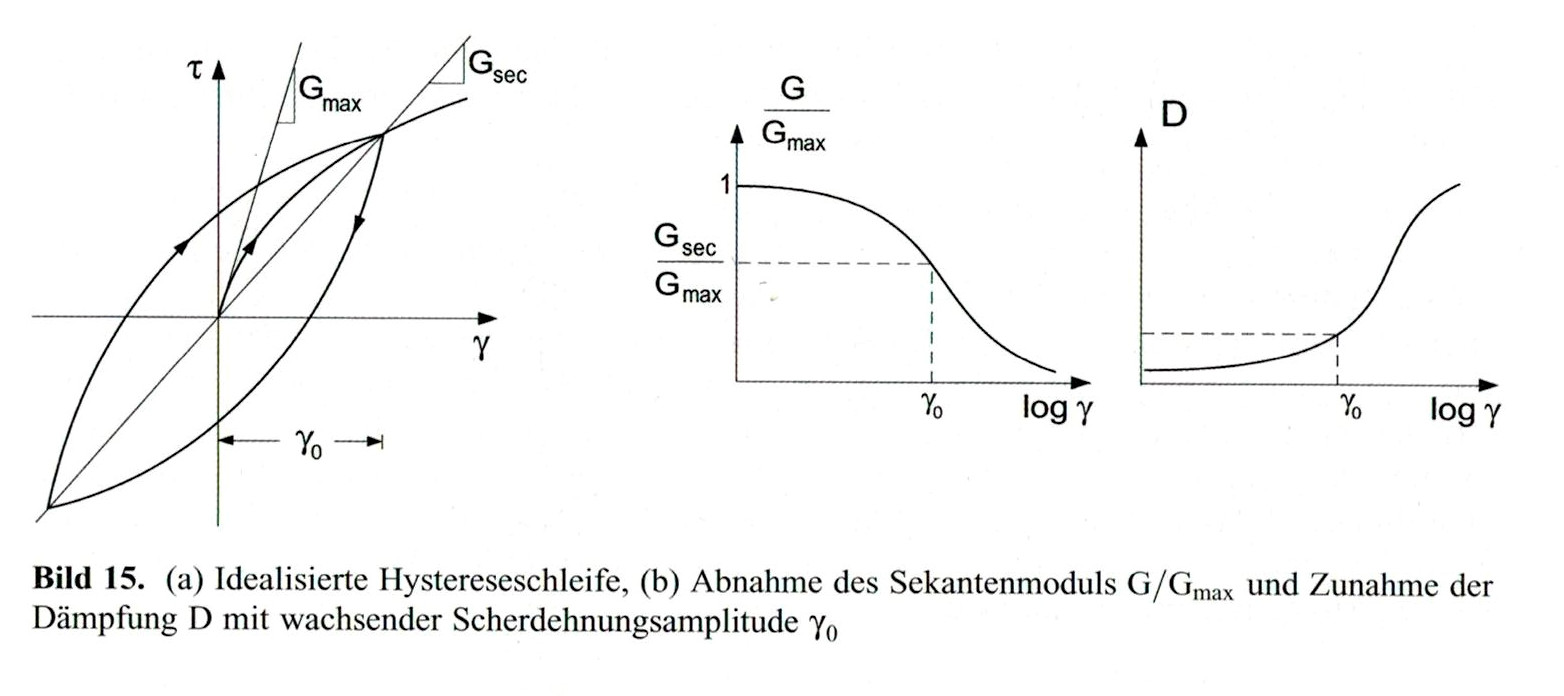
\includegraphics[width=\linewidth]{fig_img/bild15.jpg}
\caption*{Solange keine plastischen Verformungen gesucht werden,
wird angenommen, dass sich ein stationärer Zustand nach einigen Lastzyklen eingestellt hat \cite{Vrettos2017}.} 
\end{figure}
\end{frame}


\begin{frame}
\frametitle{Parameterabhängigkeit}
\begin{columns}
\begin{column}[t]{.475\linewidth}
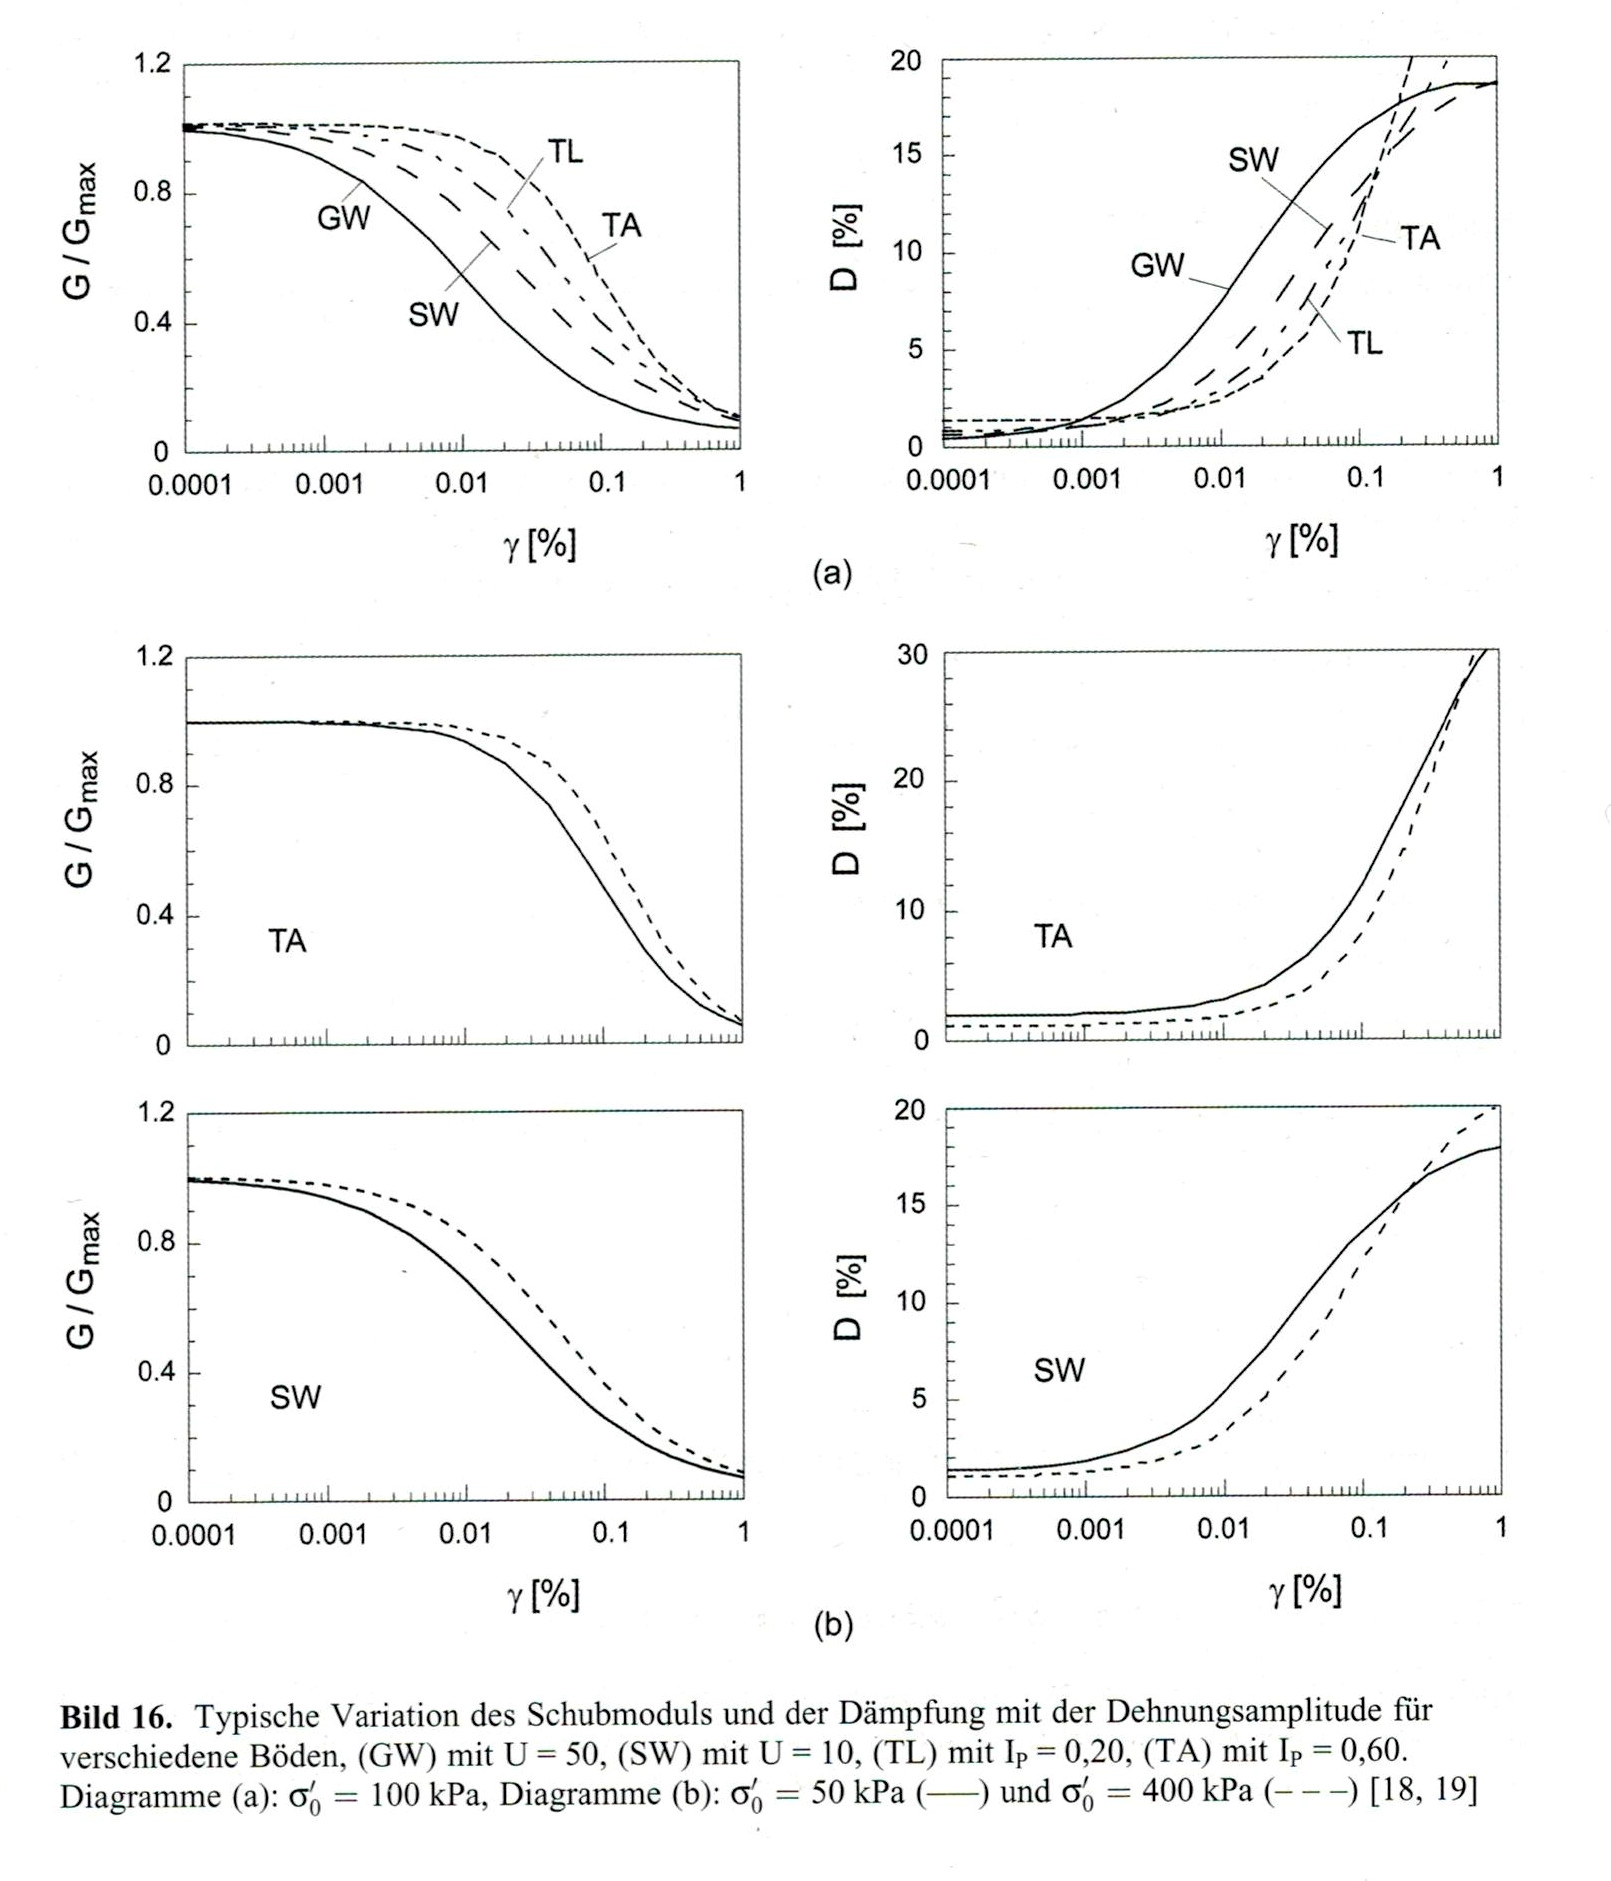
\includegraphics[width=\linewidth]{fig_img/bild16.jpg}
\end{column}
\begin{column}[t]{.525\linewidth}
\vspace{-5cm}

Schubmodul und Dämpfung werden -- außer von der Dehnungsamplitude -- vornehmlich von folgenden Parametern beeinflusst: effektives Druckniveau, Porenzahl, Plastizitätszahl, Überkonsolidierungsgrad bei bindigen Böden sowie Anzahl der Zyklen \cite{Vrettos2017}.
\end{column}
\end{columns}
\end{frame}

\begin{frame}
\frametitle{Einfache hysteretische Modelle}
\begin{figure}
\centering
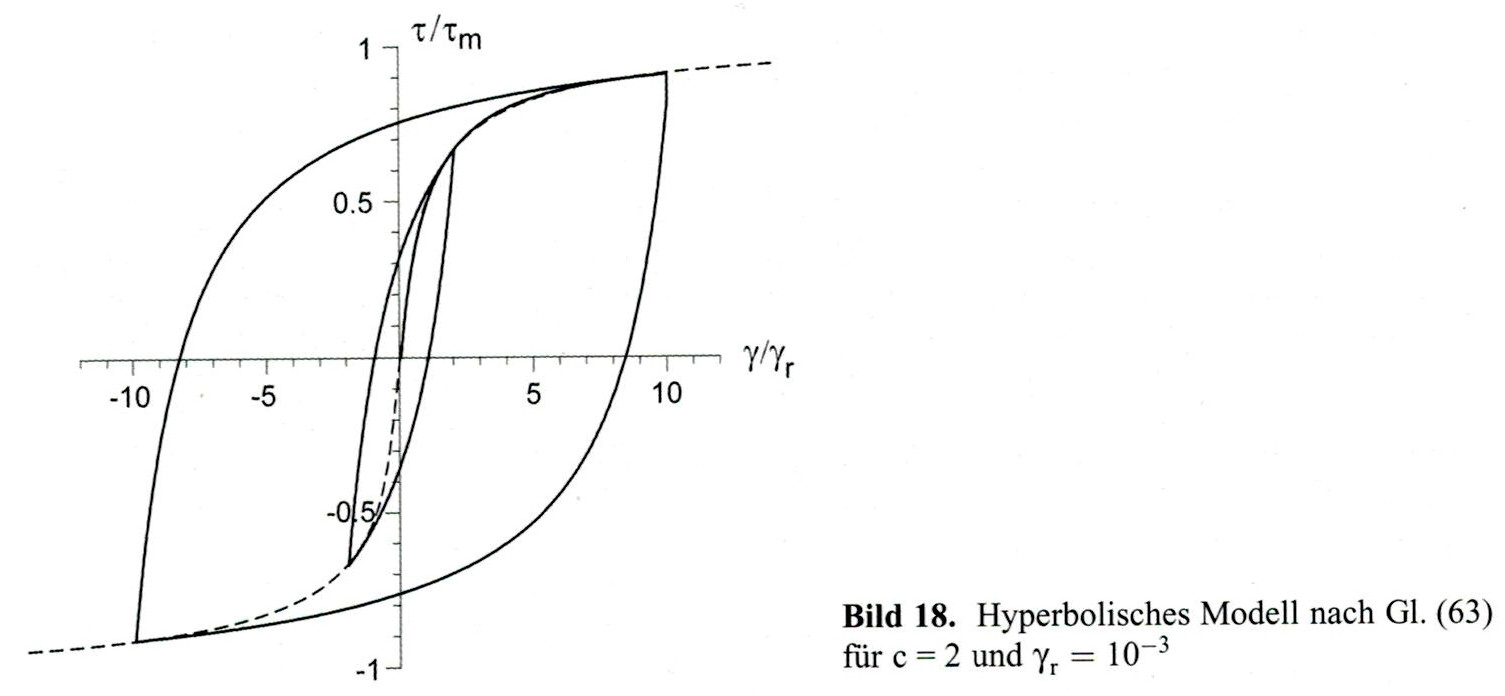
\includegraphics[width=0.95\linewidth]{fig_img/bild18.jpg}
\caption*{Gleichung (61) beschreibt die Skeleton-Kurve (gestrichelt)
und Gleichung (63) die Konstruktion der Spannungs-Dehnungsbeziehung
\cite{Vrettos2017}.} 
\end{figure}
\end{frame}

\begin{frame}
\frametitle{Einfache hysteretische Modelle}
Zur Beschreibung des Bodenverhaltens stehen grundsätzlich zwei Alternativen zur Auswahl \cite{Vrettos2017}:
\begin{itemize}
 \item Entwicklung eines Modells, womit das hysteretisch-plastische Stoffverhalten innerhalb jedes Belastungszyklus beschrieben wird. 
 \item Aufstellung eines empirischen Akkumulationsmodells, das die wesentlichen Parameter beinhaltet, ohne jedoch die Vorgänge in jedem Zyklus zu beschreiben.
\end{itemize}
\end{frame}

\begin{frame}
\frametitle{Zusatzmaterial} % online courses
\vfill
\begin{center}

\includegraphics[width=0.2\textwidth]{fig_img/youtube.png}  

\href{https://www.youtube.com/watch?v=01_KWg3QriE}{\textsl{Office Hours: CEEN 545 - Lecture 18 - Dynamic Soil Properties (Part 1)}}

\href{https://www.youtube.com/watch?v=Mngr3tujIjM}{\textsl{Office Hours: CEEN 545 - Lecture 19 - Dynamic Soil Properties (Part 2)}}
\end{center}  
\vfill
Die Reihenfolge der Videos (Teil 1: Experimentelle Parameterbestimmung, Teil 2: Mathematische Modelle) ist andersrum als in dieser Vorlesung und enthält einige Vorgriffe, nichtsdestotrotz lohnt sich schon jetzt ein Blick in Teil 2.

\end{frame}

